\documentclass[12pt, spanish]{article}
\usepackage[spanish]{babel}
\selectlanguage{spanish}
\usepackage{natbib}
\usepackage{url}
\usepackage[utf8x]{inputenc}
\usepackage{graphicx}
\graphicspath{{images/}}
\usepackage{parskip}
\usepackage{fancyhdr}
\usepackage{vmargin}

\usepackage[default]{sourcesanspro}

\setmarginsrb{2 cm}{1 cm}{2 cm}{2 cm}{1 cm}{1.5 cm}{1 cm}{1.5 cm}

\title{Análisis de Empresa:\\
Twitter, Inc. 
\includegraphics[scale = 0.05]{twitter_logo.png}  }                           
\author{Jose Luis Gallego Peña \\
María Sánchez Marcos \\
Antonio David Villegas Yeguas}                             
\date{\today}                                           

\renewcommand*\contentsname{hola}

\makeatletter
\let\thetitle\@title
\let\theauthor\@author
\let\thedate\@date
\makeatother

\pagestyle{fancy}
\fancyhf{}
\rhead{\theauthor}
\lhead{\thetitle}
\cfoot{\thepage}

\begin{document}
%%%%%%%%%%%%%%%%%%%%%%%%%%%%%%%%%%%%%%%%%%%%%%%%%%%%%%%%%%%%%%%%%%%%%%%%%%%%%%%%%%%%%%%%%

\begin{titlepage}
    \centering
    \vspace*{0.5 cm}
    
\includegraphics[scale = 0.50]{ugr.png}\\[1.0 cm]
    %\textsc{\LARGE Universidad de Granada}\\[2.0 cm]   
    \textsc{\large 1ºA}\\[0.5 cm]            
    \textsc{\large Grado en Ingeniería Informática}\\[0.5 cm]              
    \rule{\linewidth}{0.2 mm} \\[0.4 cm]
    { \huge \bfseries \thetitle}\\
    \rule{\linewidth}{0.2 mm} \\[1.5 cm]
    
    \begin{minipage}{0.4\textwidth}
        \begin{flushleft} \large
            \emph{Autores:}\\
            \theauthor
            \end{flushleft}
            \end{minipage}~
            \begin{minipage}{0.4\textwidth}
            \begin{flushright} \large
            \emph{Asignatura: \\
            Ingeniería, Empresa y Sociedad}                   
        \end{flushright}
    \end{minipage}\\[1 cm]
  	
    {\large \thedate}\\[1 cm]
 	
    \vfill
    
\end{titlepage}

%%%%%%%%%%%%%%%%%%%%%%%%%%%%%%%%%%%%%%%%%%%%%%%%%%%%%%%%%%%%%%%%%%%%%%%%%%%%%%%%%%%%%%%%%

\tableofcontents
\pagebreak

%%%%%%%%%%%%%%%%%%%%%%%%%%%%%%%%%%%%%%%%%%%%%%%%%%%%%%%%%%%%%%%%%%%%%%%%%%%%%%%%%%%%%%%%%

\section{Introducción}

Twitter es un servicio de \textit{microblogging}, con sede en San Francisco, California, con filiales en San Antonio (Texas) y Boston (Massachusetts) en Estados Unidos. Twitter, Inc. fue creado originalmente en California, pero está bajo la jurisdicción de Delaware desde 2007. 

Fue creado por Jack Dorsey en marzo de 2006, y lanzado en julio del mismo año. Desde entonces la red ha ganado popularidad mundial y se estima que tiene más de 500 millones de usuarios, generando 65 millones de tuits al día y maneja más de 800.000 peticiones de búsqueda diarias. Ha sido denominado como el "SMS de Internet".

Por tanto, en este trabajo nos centraremos en analizar \textbf{\textit{Twitter, Inc.}} como empresa, usando para ello los conocimientos aprendidos en la asignatura \textit{Ingeniería, Empresa y Sociedad} del primer curso del Grado en Ingeniería Informática por la UGR.


\begin{table}[!htb]
\centering
\begin{tabular}{l|r}
Item & Quantity \\\hline
Cosa1 & 99 \\
Cosa2 & 10
\end{tabular}
\caption{\label{tab:widgets}Tabla de ejemplo}
\end{table}

\newpage

\section{La empresa: Elementos y funciones}

La empresa es una organización que transforma un conjunto de recursos físicos, monetarios y cognitivos en bienes y/o servicios, con el objetivo principal de obtener beneficios \cite{}
Atendiendo a esta definición podemos efectivamente definir a Twitter como una empresa, y por tanto en los siguientes subapartados vamos a clasificarla atendiendo a varios criterios:

\subsection{Tamaño}

Según el tamaño tenemos que Twitter es una empresa grande ya que, según datos de 2015, tiene un total de 3.638 trabajadores y un total de ingresos de 2 mil millones de dólares.

\subsection{Sector}

Al tratarse de una empresa que ofrece servicios al público general, y ni extrae materias primas ni las transforma, podemos encasillarla en el sector terciario o sector servicios.

\subsection{Ámbito geográfico de actividad}

Su sede está en San Francisco (California), sin embargo opera en todo el mundo y ofrece gran variedad de idiomas para que cualquier persona del mundo pueda acceder a ella, por tanto estamos hablando de una empresa internacional.

\subsection{Forma jurídica}

Twitter tiene la estructura de Sociedad Anónima, es decir, está estructurada en acciones que cualquiera puede comprar e invertir en ella.

\subsection{Procedencia del capital}

Desde el año 2013 (5 años después de que la red se lanzase) Twitter es una empresa de capital abierto debido a la realización de una Oferta Pública Inicial, sin embargo es como tal una empresa privada ya que el capital es privado, pertenece a accionistas y no al estado.

\section{Dirección y gobierno de la empresa: funciones y niveles}

La función de dirección consiste en gestionar todo el funcionamiento de la empresa para conseguir alcanzar los objetivos empresariales. Para ello es imprescindible que los directivos, personas al cargo de cada tarea y con autoridad, tengan además las capacidades de motivación, liderazgo y comunicación.

En el caso de Twitter, Inc. la función de dirección comprende varios equipos con distintas funciones.

\subsection{Propiedad}

La estructura de propiedad se relaciona con el modo en que se distribuye el capital de las empresas entre sus propietarios legales (accionistas en este caso). La mayor parte de grupos de propiedad en Twitter son de capital industrial o empresarial, en concreto de capital riesgo, centradas en financiar a empresas con alto potencial de crecimiento, pero también hay gran presencia de particulares. Tenemos los siguientes accionistas principales:

\begin{itemize}

\item Kleiner Perkins Caufield and Bayers
\item Benchmark
\item Spark Capital
\item Insight Venture Partners
\item Union Square Ventures
\item Institutional Venture Partners
\item DST Global
\item Alwaleed Bin Talal

\end{itemize}

\subsection{Dirección ejecutiva}

El director ejecutivo de Twitter es Jack Dorsey, siendo también es co-fundador de esta. Además, Ed Ho y Kayvon Beykpour son gerentes generales.


La función principal de la dirección ejecutiva es actuar como cabeza visible de la empresa, informando sobre los objetivos, logros o participación de la empresa, así como gestionando la organización y los empleados.

\subsection{Equipo de Recursos Tecnológicos}



\section{Análisis DAFO}

       %Temas 1, 2 y 3 

%TEMA 4

\section{La organización en Twitter, Inc.}

La función de organización se basa, principalmente, en dividir el trabajo, tanto humano como material, para posteriormente coordinar las distintas tareas de forma agrupada para la correcta ejecución de los planes establecidos. Para esta organización debemos tener en cuenta distintos factores, como la misión, los objetivos de la empresa, el uso de herramientas para la construcción de esta estructura, entre otros.

Twitter, Inc. mantiene, claramente, una estructura adhocratica, debido a su complejidad y a su dinamismo.

En la empresa que analizamos, Twitter, Inc., ya hemos mencionado anteriormente algunos de estos (como la misión).

\newpage

\subsection{Organigrama.}

\begin{figure}[!htb]
\centering
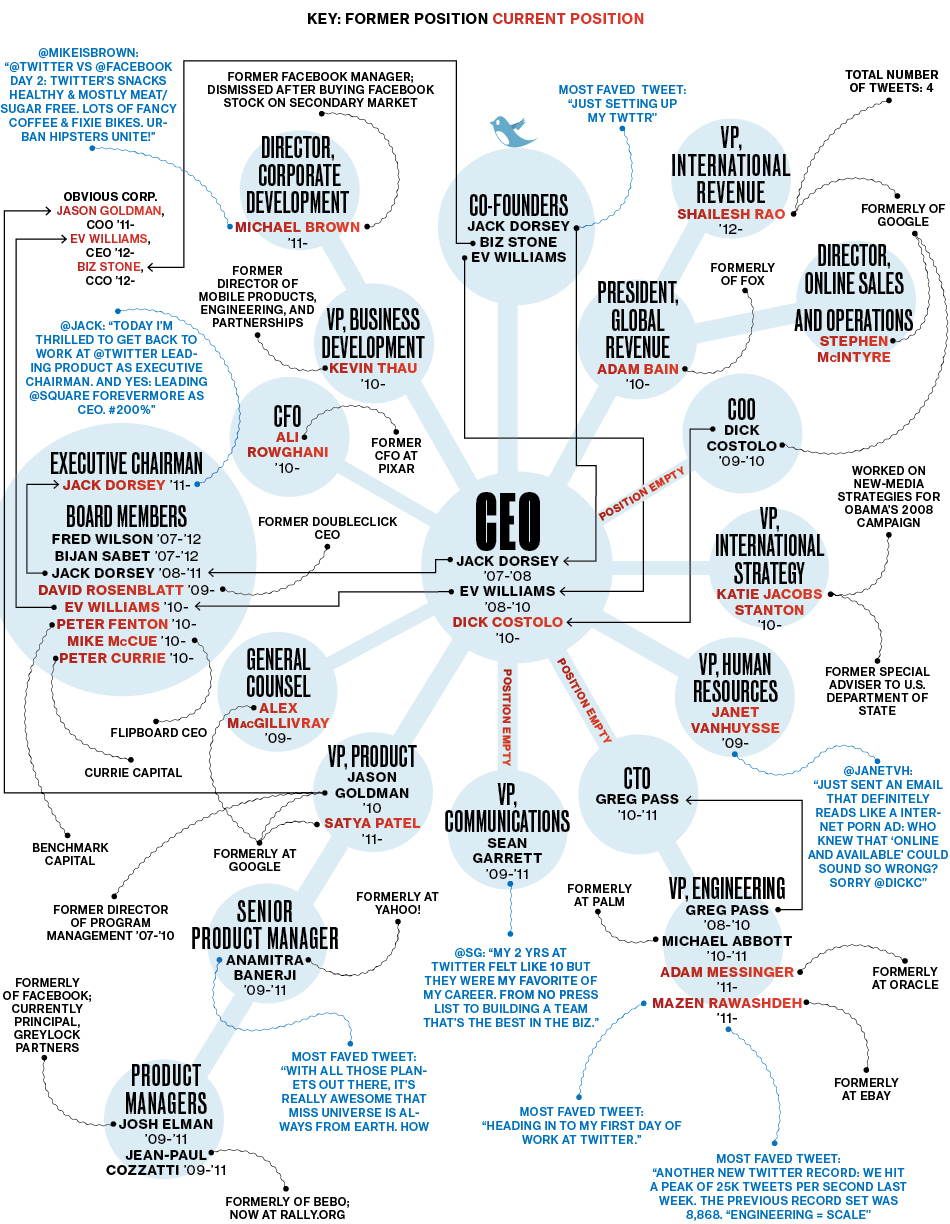
\includegraphics[scale=0.2]{organigrama.jpg}
\caption{\label{fig:frog}Organigrama Twitter, Inc. 2012}
\end{figure}


\subsection{Principios organizativos fundamentales.}

\subsubsection{Principio de la división del trabajo.}

Siguiendo estos principio, Twitter, Inc., se distribuye en distintos equipos de trabajo, entre los que se encuentran:\\

\textbf{Equipo Construir el producto}

El grupo \textit{Build the product} comprende los siguientes equipos:

\begin{itemize}

\item \textit{Data Science and Analytics}

Encargado de comprender como el mundo utiliza Twitter y como son sus usuarios.

\item \textit{Infraestructure Engineering}

Encargado de innovar, construir y mantener la infraestructura y servicios de Twitter operativos.

\item \textit{Product}

Encargado de desarrollar el producto principal, Twitter.

\item \textit{Software Engineering}

Encargado de desarrollar todos los servicios necesarios  en los que se basa Twitter, como por ejemplo Bootstrap.

\item \textit{User Services}

Encargado de dar soporte a los usuarios de Twitter siempre que lo necesiten.

\item \textit{Design and Research}

Encargados de mantener el diseño y características de Twitter a la última.

\end{itemize}

\textbf{Equipo Seguir manteniéndonos}

El grupo \textit{Keep us running} comprende los siguientes equipos:

\begin{itemize}

\item \textit{Finance}

Encargado de controlar las finanzas de Twitter, haciendo posible que sus productos sean rentables.

\item \textit{Legal and Public Policy}

Encargado de defender legalmente a la compañía y a sus usuario. 

\item \textit{People}

Encargado de los Recursos Humanos de Twitter, intentando que sea un lugar serio a la vez que agradable para trabajar.

\item \textit{Workplace}

Encargado de que las oficinas de Twitter sean lo más cómodas y útiles, para un correcto desarrollo de sus empleados.

\end{itemize}

\textbf{Equipo Promover el negocio}

El grupo \textit{Promote the business} comprende los siguientes equipos:

\begin{itemize}

\item \textit{Marketing and Communications}

Encargado de enseñar al mundo los avances realizados en Twitter.

\item \textit{Sales and Partnerships}

Encargado de trabajar en conjunto con otras marcas y compañías para alcanzar sus objetivos de forma conjunta y más sencilla.

\end{itemize}

\textbf{Equipo Nuestras marcas}

El grupo \textit{Our family of brands} comprende los siguientes equipos:

\begin{itemize}

\item \textit{Periscope}
\item \textit{MoPub}\\

\end{itemize}



Todos estos equipos se distribuyen entre más 35 países alrededor del mundo.

\subsubsection{Principio de la especialización del trabajo.}

Como vemos en el apartado anterior, existen grandes distinciones entre los distintos equipos de trabajo, por lo que es necesaria una especialización, que dependerá de cada equipo, encontrando así un alto nivel de especialización en cada uno de ellos.

\subsubsection{Principio de jerarquía, unidad de mando y ámbito de control.}

Estos principios, explicados y revisados en apartados anteriores, suponen una correcta organización del trabajo, esencial para el desarrollo de los objetivos de la empresa.

\subsubsection{Principio de descentralización.}

Como hemos visto, en Twitter, Inc. vemos una clara descentralización con los distintos grupos de trabajo, sin obviar las decisiones tomadas por los altos directivos.

\subsection{Adoctrinamiento y preparación de los empleados.}

Twitter, Inc. sigue un claro ejemplo de adoctrinamiento departamental, en el que prepara a sus empleados según el departamento al que pertenezcan, ya que, como hemos visto, su separación en equipos hace que esto sea más fácil de realizar.


\subsection{Factores de contingencia.}

\subsubsection{Entorno.}

En Twitter, Inc. encontramos un entorno dinámico, debido al constante cambio tecnológico, vemos una gran incertidumbre, lo que hace más difícil predecir cambios en el entorno, ademas, presenta un entorno complejo, ya que es necesario un alto nivel de formación, conocimiento, y habilidades para resolver los problemas planteados durante el desarrollo de la empresa.

\subsubsection{Edad.}

Twitter, Inc. fue fundada en 2006, esto hace que su organización no este aún muy consolidada, debido a la falta de madurez, aunque esto podría interpretarse como algo positivo, ya que permite adaptarse a la complejidad y dinamismo del entorno.

\subsubsection{Tamaño.}

En los últimos años, sobre todo desde 2012, Twitter, Inc., ha sufrido un fuerte crecimiento en su base de usuarios, lo que le ha permitido crecer de forma significativa su tamaño como empresa.

Actualmente, Twitter, Inc. cuenta con 336 millones de usuarios activos (datos del primer cuatrimestre de 2018) y con 3.372 empleados (2017).

\subsubsection{Tecnología.}

El principal desarrollo de Twitter, Inc. como empresa se basa en el desarrollo tecnológico, por lo que vemos que este tiene un gran impacto, tanto a nivel administrativo como económico dentro de la empresa, y esto lo podemos ver en la importancia de sus departamentos, la mayoría centrados en desarrollo de software, y en sus distintas tecnologías, usadas para apoyarse en el desarrollo de su aplicación principal, Twitter, como por ejemplo, Bootstrap, Gizzard Scala, FlockDB, entre otros.


\subsubsection{El entorno y la organización.}

En Twitter, Inc. encontramos un en entorno diversificado, ya que Twitter, Inc. se tiene que adaptar a distintos tipos de clientes, zonas geográficas, etc, para dar a conocer y expandir su producto. Ademas, el entorno es competitivo, ya que vemos como cada día surgen nuevas empresas competidoras, o ha de competir con otras con experiencia, como pueden ser Facebook, Instagram, Snapchat, etc, sumando el que al ser de tipo tecnológico, el alto nivel de incertidumbre impida reconocer posibles futuros competidores.

\subsection{La estructura de Twitter, Inc.}

Twitter, Inc. presenta claramente una estructura adhocrática, ya que, como hemos visto en el organigrama y en al analizar la dirección ejecutiva de la empresa, la parte más importante de Twitter, Inc. es el ápice estratégico y el núcleo operativo, pudiendo considerar este último como "doble", uno trabajando en los proyectos principales, como Twitter o Periscope, y el segundo núcleo de operaciones, que se alterara según sea necesario para la realización de otros proyectos, un ejemplo serian los ya mencionados como   Bootstrap, Gizzard Scala o FlockDB.





%TEMA 5

\section{El entorno en Twitter, Inc.}
%TODO


%TEMA 6

\section{La dirección estratégica en Twitter, Inc.}

La estrategia representa la relación entre la empresa con su entorno y las acciones que emprende para realizar sus objetivos, haciendo un uso racional de sus recursos, con el objetivo de mejorar el rendimiento de la empresa.

El proceso de dirección estratégica consta de tres partes.

\subsection{Análisis estratégico.}

Se realiza un análisis de la misión y los objetivos de la empresa, junto con un análisis tanto externo como interno de esta (DAFO) y de los objetivos de propietarios y stakeholders.

\subsection{Formulación de estrategias.}

Una vez realizados los análisis previos, la empresa propone alternativas u opciones estratégicas  que deben ser consideradas tanto a nivel operativo, como a nivel funcional.

Twitter, Inc., en varias ocasiones ha formulado distintos tipos de estrategias.

\subsubsection{Estrategias competitivas.}

Para hacer frente a sus rivales, intentando remodelar sus productos, haciéndolos más atractivos y útiles de cara al público, como por ejemplo, la implementación de contenido personalizado a cada usuario, o el avance en la interacción de usuarios en su principal servicio, Twitter.

\subsubsection{Estrategias corporativas.}

Planteando la expansión de su negocio, con plataformas como Periscope, o MoPub, que han permitido a Twitter, Inc. crecer a nivel corporativo, y mantener la atención, tanto de competidores como de posibles stakeholders, gracias la diversidad de productos que le ha aportado estas estrategias corporativas.

\subsection{Implantación de la estrategia.}

Una vez formulada la estrategia, esta ha de implantarse en todos los niveles de la empresa, para cumplir con su objetivo, obtener una ventaja competitiva, algo que Twitter, Inc. consiguió con respecto a otras empresas del sector, lo que condujo a una mayor penetración en el mercado y el cumplimiento de su Misión y objetivos.




 %Temas 4, 5, 6 y 7
\section{Gestion financiera}

\subsection{El negocio de Twitter}

El negocio de Twitter es bastante simple y consta de 3 segmentos:

\begin{itemize}


\item Usuarios: la propuesta de valor de Twitter consisten en ofrecer a su masa crítica de usuarios 
servicios de microblogging y la posibilidad de mantenerse actualizado de lo que sucede en el 
mundo  al  instante  a  través  de  diversos  canales  como  su  app  para  smartphones,  su  página 
web, y las APIs que permiten integrar Twitter en otras webs. 
Twitter no genera ingresos de manera directa con sus usuarios.

\item Empresas: Aprovechando la masa crítica de usuarios existentes, y la información que posee 
de  los  mismos,  Twitter  ofrece  servicios  de  publicidad  a  empresas,  que  pueden  mostrar  su 
publicidad a aquellos usuarios con mayor probabilidad  de  comprar  productos  de  esas 
empresas (Targeted  Marketing). Estos servicios de Marketing incluyen: tweets 
promocionados (el anunciante paga por mostrar el tweet a un segmento de usuarios 
definido), cuentas promocionadas (el anunciante paga por adquirir seguidores) y tendencias 
promocionadas (el anunciante paga por tener más visibilidad como "trending topic"). 
Twitter obtiene ingresos de este segmento de clientes.

\item Desarrolladores: Twitter permite además a desarrolladores la posibilidad de conectarse a 
Twitter para generar herramientas relacionadas con analítica web, u otras apps que ayuden a 
hacer crecer la masa crítica de usuarios que utilizan Twitter. Esto aumenta los ingresos de Twitter de manera indirecta. El modelo de negocio de Twitter es un modelo de negocio bilateral, que se basa captar por un lado a usuario que generen actividad y compartan información para su plataforma, y  captar anunciantes por el otro, aprovechando su plataforma y la información generada por sus usuarios para vender servicios de publicidad. Es decir que Twitter actúa como intermediario, como si de una plataforma  de  publicidad  se  tratase.


\end{itemize}

Por tanto, Twitter será rentable en la medida en la que lo sea para sus anunciantes.
Twitter necesita que el valor de cada usuario a lo largo de su vida sea mayor que su coste de adquisición.

\newpage

\subsection{Ingresos y pérdidas (2018)}

\begin{figure}[!htb]
\centering
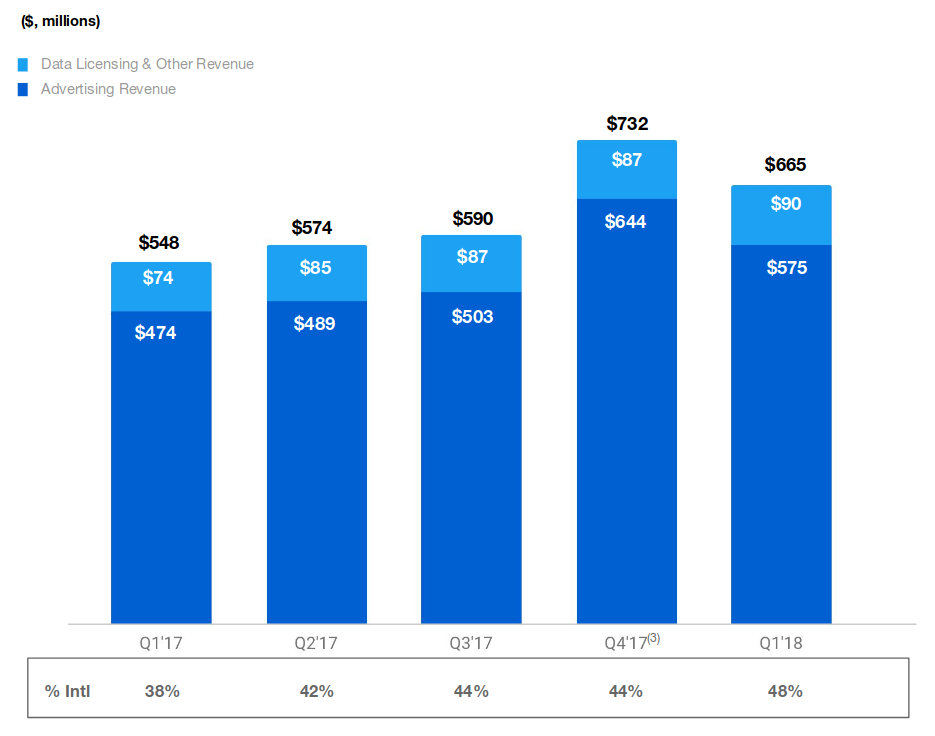
\includegraphics[scale=0.35]{revenues.png}
\caption{\label{fig:frog}Ingresos de Twitter, Inc por cuatrimestres}
\end{figure}

En esta imagen podemos observar cómo los ingresos de Twitter dependiendo de su origen (Licencia de datos, ingresos por publicidad y otros ingresos)


\begin{figure}[!htb]
\centering
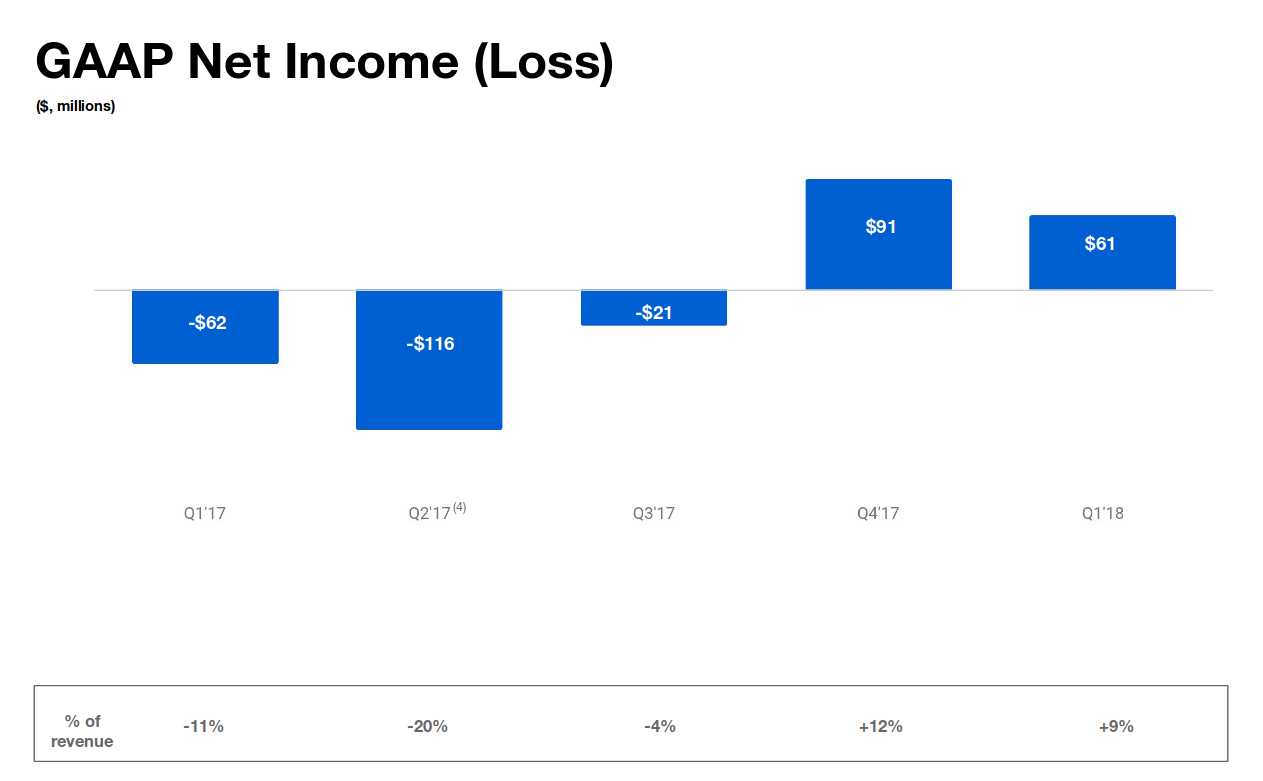
\includegraphics[scale=0.25]{loss.png}
\caption{\label{fig:frog}Ingresos netos de Twitter, Inc por cuatrimestres.}
\end{figure}


Podemos observar cómo los ingresos netos de Twitter Inc. durante comienzos de 2017-2018, fuerosn enteramente negativos.

\subsection{Activos.}

\subsubsection{Activos no corrientes.}

Para Twitter, Inc. los activos no corrientes corresponden a toda su infraestructura de servidores, software, patentes, licencias y datos obtenidos en sus productos.

\subsubsection{Activos corrientes.}

Corresponden al conjunto de bienes de la empresa, en este caso, corresponderá a una parte pequeña de los activos, aunque se espera un crecimiento en esta, ya que como hemos comentado, Twitter, Inc. se encuentra en una etapa de madurez a nivel empresarial, lo que resultara en una generación de beneficios.


\subsection{Recursos financieros.}

\begin{figure}[!htb]
\centering
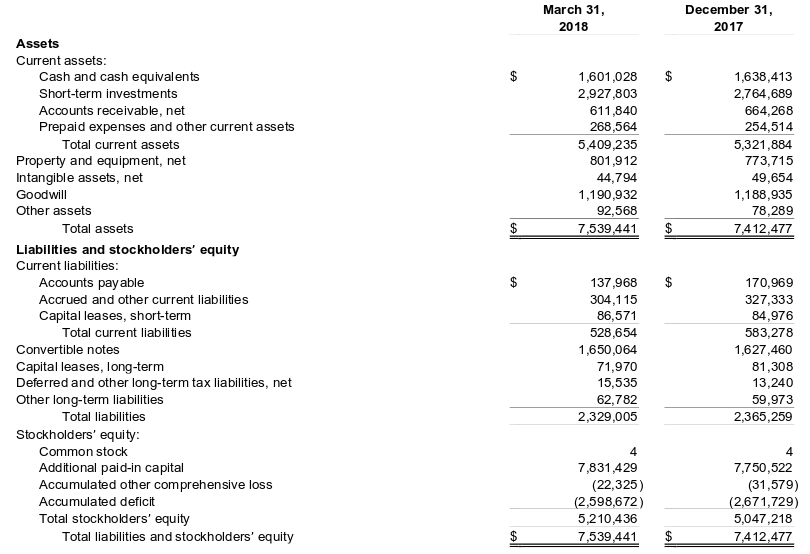
\includegraphics[scale=0.6]{ingresos.png}
\caption{\label{fig:frog}Diferencia de ingresos de Twitter, Inc.}
\end{figure}

\subsubsection{Recursos financieros propios.}

Como vemos en la imagen de ingresos de Twitter, Inc. , menos de la mitad de ingresos que usa Twitter, Inc. son generados  por la empresa, esto es causado por el ámbito de esta, ya que normalmente, en las empresas de ámbito tecnológico el valor de la empresa viene dado por la importancia que el sector le de a esta, ya que los propios productos no pueden ser evaluados de forma física.

\subsubsection{Recursos financieros externos.}

La inversión de agentes externos en la empresa tiene una gran importancia, de ahí que se generen grandes conflictos de intereses en Twitter, Inc. , los valores de la compañía difieren con los valores de los stakeholders, aunque la estructura organizativa permita lidiar con estos.

\subsubsection{Fondo de maniobra.}

Observamos como el fondo de maniobra ha sido muy importante para Twitter, Inc. ya que ha permitido mantener la empresa en su etapa anterior, en la que no era capaz de generar ingresos netos. Se espera que en un periodo de tiempo próximo (a corto plazo) este fondo se amplié gracias al comienzo de generación de ingresos.

\section{Recursos Humanos}

A grandes rasgos, los recursos humanos de una empresa son el conjunto de empleados y colaboradores que
trabajan en la empresa, aunque comunmente nos referimos a ellos como el proceso de reclutamiento, selección, formación, evaluación, compensación... de una empresa. Normalmente, estas políticas son llevadas a cabo por un departamento en específico dentro de la empresa.

\subsection{Reclutamiento}

En Twitter, el reclutamiento es un proceso muy sencillo, ya que en su misma página principal te dan la opción de presentarte para poder trabajar con ellos en sus diferentes departamentos en sucursales de todo el mundo.


\includegraphics[scale=0.25]{reclutamiento1.png}
\newpage

Una vez accedida a esta sección, decides a qué departamento quieres aplicar para pasar al proceso de selección.


\includegraphics[scale=0.25]{reclutamiento2.png}

\subsection{Selección}

El proceso de selección en twitter consta de 3 pasos

\subsubsection{Paso 1}
Después de presentar la solicitud, un reclutador podría comunicarse con el solicitante para efectuar una llamada de presentación.

\subsubsection{Paso 2}
Si es del agrado del reclutador, más tarde le llamarán para entrevistas con una o dos personas más.

\subsubsection{Paso 3}
Si continua a lo largo del proceso, irá a la oficina de Twitter (En el lugar solicitado por el solicitante) una o dos veces para entrevistarse finalmente con 5-10 personas más.

\subsection{Compensación}

Twitter se preocupa del estado en el que sus empleados trabajan, por tanto, para retener el talento, se centran en dos puntos: el aprendizaje y la directiva.
En la empresa tienen organizaciones de aprendizaje de talla mundial enfocadas a Twitter. Tienen Twitter University, enfocado al desarrollo de capacidades de ingeniería móvil para los empleados de la compañía. Por otro lado, creen que la clave para la comodidad de sus empleados es que sus directores sean personas competentes y agradables, por ello, los directores de departamento reciben 6 horas de clase de dirección y motivación al trimestre, de esta manera, los directores estarán implicados y apasionados realmente en el proyecto. En Twitter Inc piensan que no se despiden puestos, sino empleados.

\subsection{Formación}

Como hemos comentado anteriormente, existe una formación interna tanto como para empleados, como para directivos llamada Twitter University.

\subsection{Socialización}

Para facilitar el proceso de adaptación de un nuevo trabajador a la empresa, Twitter ofrece en sus oficinas lugares de ocio como salones y comedores dondde los empleados pueden relacionarse y descansar tras una jornada de trabajo.

\subsection{Relaciones Laborales}

La directora de Recursos Humanos afirma que la clave del éxito en este ámbito es, sin duda, el apoyo que brindan los directores los empleados de sus proyectos, por tanto, hay una estrecha relación entre todos los trabajadores de la empresa.

\section{El Marketing}

Definimos Marketing como: $"$Conjunto de técnicas y estudios que tienen como objeto mejorar la comercialización de un producto$"$.

A continuación explicaremos cómo aborda Twitter las actividades de Marketing.

\subsection{Análisis de Mercado y comportamiento del consumidor}

Twitter se encuentra en un sector muy competitivo: las redes sociales.

Existen muchas aplicaciones de comunicación de este tipo, como Facebook, Instagram, Snapchat, Tumblr... ¿Pero qué es lo que ha hecho a Twitter destacar ante sus competidores?

Twitter se dirige a un mercado joven y dinámico, pero también con el paso del tiempo, se ha transformado en una herramienta para las empresas, tanto para promocionarse y anunciarse como para investigar el comportamiento y preferencias de su clientela.
La clave de su éxito reside en la facilidad de uso que tiene (tanto para publicar tu propio contenido como para interactuar con el contenido ajeno), la posibilidad de personalización, el uso de los llamados \textit{hashtags} para agrupar contenidos, la ausencia de censura exceptuando 5 países y, para atraer visitas y ver de qué se habla en el momento, las \textit{tendencias}.

Nuestra empresa ha sabido localizar el centro de su público y darles las herramientas necesarias para expresarse libremente y de forma segura.

\subsection{Estrategia de Marketing}

La nueva estrategia de Marketing de Twitter incluye vídeos explicando los valores que lo distinguen de las otras plataformas. Este esfuerzo se deriva de la investigación que la compañía reveló. Mientras que el 90\% de las personas reconocían globalmente la marca Twitter, no lo usaban porque no entendían qué era Twitter. La compañía busca ahora cambiar la percepción de que Twitter es una red social qu permite a los usuarios conectarse con familiares y amigos para convertirse en un lugar activo para descubrir noticias.

Twitter se está posicionando como plataforma única donde se pueden acceder tanto a noticias de grandes eventos, hasta noticias locales junto con comentarios en directo.

Esta estrategia que destaca su singularidad atraerá a más público, afirma la directora de Marketing.

También están haciendo convenios con compañías como Samsung para que su aplicación venga instalada de forma predeterminada en sus dispositivos.       %Tema 8, 9 y 10 


\newpage

\bibliographystyle{plain}
\bibliography{biblist}

\end{document}